\noindent \textred{1.} First use the iteration method to solve the recurrence, draw the recursion tree to analyze.
$$ T(n) = T(\frac{n}{2}) + 2T(\frac{n}{8}) + n^2 $$
Then use the substitution method to verify your solution.
\newline \\
\textblue{Analysis with recursion tree:
\begin{figure}[!h]
    \centering
    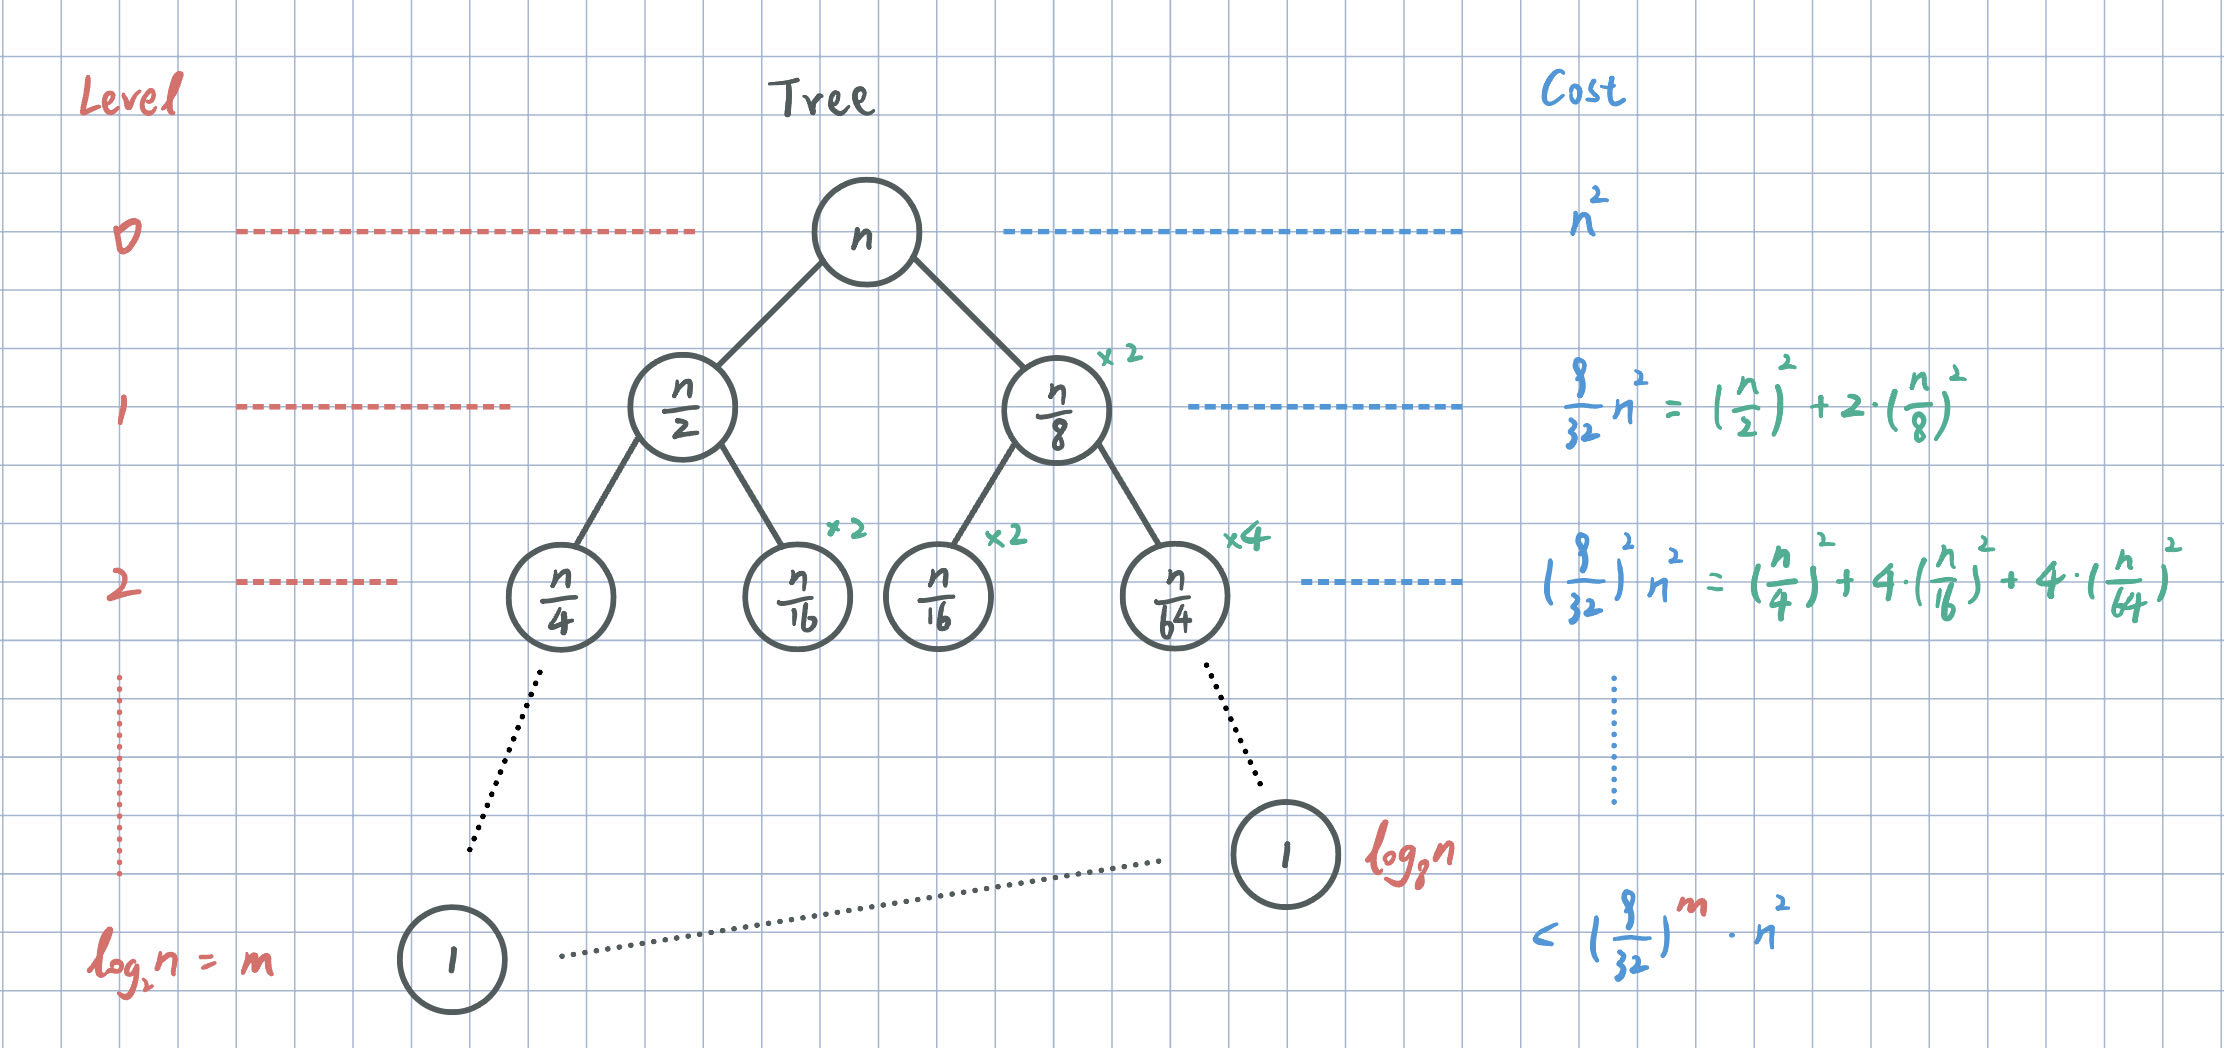
\includegraphics[width=\linewidth]{HWs/HW2/HW02_01.jpg}
    % \label{fig:HW02_01_tree}
\end{figure}
\[
\begin{aligned}
    T(n) &< [1 + \frac{9}{32} +  (\frac{9}{32})^2 + \cdots +  (\frac{9}{32})^{\log_2 n}] \cdot n^2 \\
    &< [1 + \frac{9}{32} +  (\frac{9}{32})^2 + \cdots +  (\frac{9}{32})^{+\infty}] \cdot n^2 \\
    &= \frac{1}{1- 9/32} \cdot n^2 \implies \underline{T(n) = O(n^2)}
\end{aligned}
\]
\newline \\
Verify with substitution method: \\
Assume $T(k) \leq c \cdot k^2, ~\forall k < n$, we have
\[
\begin{aligned}
    T(n) &= T(\frac{n}{2}) + 2T(\frac{n}{8}) + n^2 \\
    &\leq c \cdot (\frac{n}{2})^2 + 2c \cdot (\frac{n}{8})^2 + n^2 \\
    &= (1+\frac{9}{32}c) \cdot n^2 = \underline{O(n^2)}
\end{aligned}
\]
}